\section{Giai đoạn 3: Hệ thống đối sánh tài liệu tham khảo bằng học máy}

\subsection{Phát biểu bài toán xếp hạng ứng viên và thiết kế dữ liệu nhãn}

Trong cấu trúc kho dữ liệu học thuật sau hai giai đoạn đầu, mỗi bài báo trích dẫn $p$ sở hữu đồng thời một tập gồm $m_p$ mục thư mục BibTeX chuẩn hóa $\mathcal{E}_p = \{e_1, \dots, e_{m_p}\}$ trích xuất từ mã nguồn LaTeX và một tập gồm $n_p$ tài liệu tham khảo có định danh arXiv $\mathcal{R}_p = \{r_1, \dots, r_{n_p}\}$ thu hoạch từ đồ thị tri thức học thuật. Bài toán đối sánh tài liệu tham khảo được phát biểu dưới dạng phân giải thực thể nội bài báo trên không gian ứng viên tích Đề-các $\mathcal{E}_p \times \mathcal{R}_p$. Với mỗi mục truy vấn $e_i \in \mathcal{E}_p$, mô hình cần ước lượng hàm chấm điểm $f(e_i, r_j)$ cho từng ứng viên $r_j \in \mathcal{R}_p$ sao cho tài liệu tham khảo đúng $r^*_i$ (khi tồn tại trong $\mathcal{R}_p$) đạt thứ hạng cao nhất trong danh sách sắp xếp giảm dần, ưu tiên vị trí dẫn đầu trong nhóm năm ứng viên hàng đầu. Việc thu hẹp không gian ứng viên về phạm vi nội bài báo giúp giảm số ứng viên trung bình xuống còn vài chục tài liệu thay vì hàng trăm nghìn bản ghi toàn kho. Tuy nhiên, phạm vi nội bài báo lại tạo ra bài toán phân biệt tinh vi giữa các công trình cùng chủ đề, cùng nhóm tác giả hoặc các chuỗi bài báo nhiều phần thường được trích dẫn cạnh nhau trong một văn bản khoa học. Nhằm tuân thủ tuyến đánh giá chuẩn độc lập không dùng mô hình ngôn ngữ lớn hay vector nhúng huấn luyện sẵn theo quy định học phần~\cite{hcmus_intro_ds}, hệ thống đối chiếu trực tiếp hai họ học máy có cơ chế tối ưu bổ trợ nhau: phân loại nhị phân điểm-theo-điểm bằng Hồi quy Logistic cân bằng trọng số lớp~\cite{pedregosa2011} và học xếp hạng theo danh sách bằng LightGBM LambdaRank tối ưu chỉ số NDCG@5~\cite{ke2017,burges2010}.

Để xây dựng tập dữ liệu giám sát đáng tin cậy trên toàn bộ kho $N = 25{,}000$ bài báo của năm thành viên, nhóm thiết kế quy trình gán nhãn hai tầng tách biệt hoàn toàn giữa tập chuẩn thủ công và tập tự động quy mô lớn. Ở tầng thủ công, mỗi thành viên chọn độc lập $5$ bài báo từ dải dữ liệu cá nhân để lập tập chuẩn gồm $25$ bài báo với $2{,}519$ mục BibTeX và $1{,}880$ cặp đối sánh đúng đã xác minh (phân bố gồm Ngô Mẫn Nhi $882$, Trịnh Huỳnh Nhi $510$, Phạm Minh Trọng $189$, Huỳnh Huy Hoàng $157$ và Nguyễn Phúc Khang $142$ cặp khớp). Mỗi bài báo thủ công đều đạt ít nhất $26$ cặp khớp, vượt định mức tối thiểu $20$ cặp mỗi bài, còn tổng số $1{,}880$ cặp của cả nhóm vượt xa ngưỡng $500$ cặp của đề bài. Toàn bộ tập thủ công được đối chiếu hoàn toàn từ đầu mà không điền sẵn gợi ý từ bộ quy tắc tự động nhằm triệt tiêu thiên lệch xác nhận và đảm bảo tính khách quan khi kiểm định ngược. Ở tầng tự động, hệ thống lấy mẫu $500$ bài báo mỗi thành viên từ phần kho còn lại, tạo thành $2{,}500$ bài báo ($10.01\%$ trong số $24{,}975$ bài báo ngoài tập thủ công) với $98{,}922$ mục BibTeX và $33{,}493$ cặp khớp. Gộp cả hai tầng, tập dữ liệu đối sánh toàn nhóm bao gồm $2{,}525$ bài báo ($1{,}934$ bài có ít nhất một mục BibTeX và $591$ bài không có mục BibTeX) với $101{,}441$ mục được phân loại trạng thái, gồm $35{,}373$ mục có đích khớp, $65{,}816$ mục không có đích khớp trong kho tham khảo arXiv, $242$ mục chưa rà soát và $10$ mục mơ hồ.

Bộ gán nhãn tự động cho $2{,}500$ bài báo được đóng băng trước giai đoạn huấn luyện dưới dạng bộ quy tắc tất định ba tầng nhằm cân bằng giữa độ chính xác cao và độ phủ rộng. Ở tầng thứ nhất, hệ thống trích xuất mã định danh arXiv xuất hiện tường minh trong mục BibTeX rồi đối chiếu trực tiếp với tập ứng viên của bài báo. Khi một mục chứa mã arXiv tường minh nhưng mã này hoàn toàn vắng mặt trong tập tài liệu tham khảo đã thu hoạch, quy tắc áp đặt cơ chế phủ quyết cứng kết luận không khớp nhằm ngăn các tầng mờ phía sau ghép nhầm vào một bài báo khác có tiêu đề gần giống. Ở tầng thứ hai, hệ thống đối chiếu trùng khớp chính xác trên tiêu đề đã chuẩn hóa, kết hợp kiểm tra tính nhất quán chữ số cho chuỗi công trình nhiều phần và phân tách bằng họ tác giả khi có nhiều ứng viên trùng tiêu đề. Ở tầng thứ ba, các mục chưa được quyết định ở hai tầng đầu phải đạt điểm chồng lấp và bao hàm từ vựng tiêu đề tối thiểu $0.65$, sau đó được hiệu chỉnh cộng $0.08$ khi trùng họ tác giả, cộng $0.04$ khi năm công bố gần nhau và trừ $0.15$ khi năm công bố cách xa. Một cặp ứng viên ở tầng thứ ba chỉ được chấp nhận khi điểm tổng hợp đạt ít nhất $0.82$, vượt cổng biên độ mơ hồ tối thiểu $0.10$ so với ứng viên xếp thứ hai và không vi phạm điều kiện phủ quyết biến thể từ ghép.

\begin{table}[htbp]
    \centering
    \scriptsize
    \renewcommand{\arraystretch}{1.20}
    \begin{tabularx}{\textwidth}{l r r r r X}
        \toprule
        \textbf{Phân vùng} & \textbf{Tổng bài} & \textbf{Thủ công} & \textbf{Tự động} & \textbf{Truy vấn} & \textbf{Cấu trúc truy vấn có đích khớp} \\
        \midrule
        Huấn luyện (Train) & $2{,}505$ & $15$ & $2{,}490$ & $34{,}334$ & $1{,}014$ thủ công + $33{,}320$ tự động \\
        Kiểm định (Valid)  & $10$      & $5$  & $5$       & $511$      & $435$ thủ công + $76$ tự động \\
        Kiểm tra (Test)    & $10$      & $5$  & $5$       & $528$      & $431$ thủ công + $97$ tự động \\
        \midrule
        \textbf{Tổng toàn nhóm} & $\mathbf{2{,}525}$ & $\mathbf{25}$ & $\mathbf{2{,}500}$ & $\mathbf{35{,}373}$ & $\mathbf{1{,}880}$ \textbf{thủ công +} $\mathbf{33{,}493}$ \textbf{tự động} \\
        \bottomrule
    \end{tabularx}
    \caption{Phân chia tập dữ liệu đối sánh ở cấp độ bài báo theo phân tầng năm thành viên (hạt giống ngẫu nhiên $42$)}
    \label{tab:m3_split}
\end{table}

Cuộc kiểm toán độc lập bộ quy tắc tự động ba tầng trên toàn bộ $25$ bài báo thủ công cho thấy chất lượng nhãn giám sát yếu đạt độ tin cậy cao với độ chính xác $98.72\%$ và độ phủ $98.83\%$, tương ứng $1{,}858$ cặp khớp đúng, $373$ trường hợp không khớp đúng, $24$ trường hợp ghép sai và $22$ trường hợp bỏ sót. Phân rã sâu theo từng tầng quy tắc chỉ rõ bản chất sai số của bộ quy tắc: cả tầng đối chiếu trực tiếp mã định danh ($301/301$) lẫn tầng trùng khớp chính xác tiêu đề chuẩn hóa ($1{,}552/1{,}552$) đều đạt độ chính xác tuyệt đối $100\%$. Ngược lại, toàn bộ $24/24$ lỗi ghép sai xuất phát từ tầng đối sánh mờ thứ ba ($5$ đúng so với $24$ sai), còn $21/22$ lỗi bỏ sót bắt nguồn từ cơ chế phủ quyết cứng khi mã arXiv vắng mặt ($30$ không khớp đúng so với $21$ bỏ sót). Dựa trên tập $2{,}525$ bài báo đã gán nhãn, quy trình chia dữ liệu thực hiện phân chia nghiêm ngặt ở cấp độ bài báo theo chiến lược phân tầng đều năm thành viên với hạt giống ngẫu nhiên $42$ để không một bài báo trích dẫn nào xuất hiện đồng thời ở hai phân vùng. Như tổng hợp tại Bảng~\ref{tab:m3_split}, tập huấn luyện gồm $2{,}505$ bài báo ($15$ thủ công và $2{,}490$ tự động) sinh ra $34{,}334$ truy vấn có đích khớp tương ứng với $1{,}561{,}952$ cặp ứng viên huấn luyện. Trong khi đó, tập kiểm định và tập kiểm tra mỗi tập gồm đúng $10$ bài báo ($5$ thủ công và $5$ tự động, chia đều mỗi thành viên một bài thủ công và một bài tự động), cung cấp lần lượt $511$ và $528$ truy vấn với tỷ trọng nhãn thủ công áp đảo ($85.1\%$ ở tập kiểm định và $81.6\%$ ở tập kiểm tra); toàn bộ luồng xử lý của giai đoạn này được minh họa trong Hình~\ref{fig:m3_matching_pipeline}.

\begin{figure}[htbp]
    \centering
    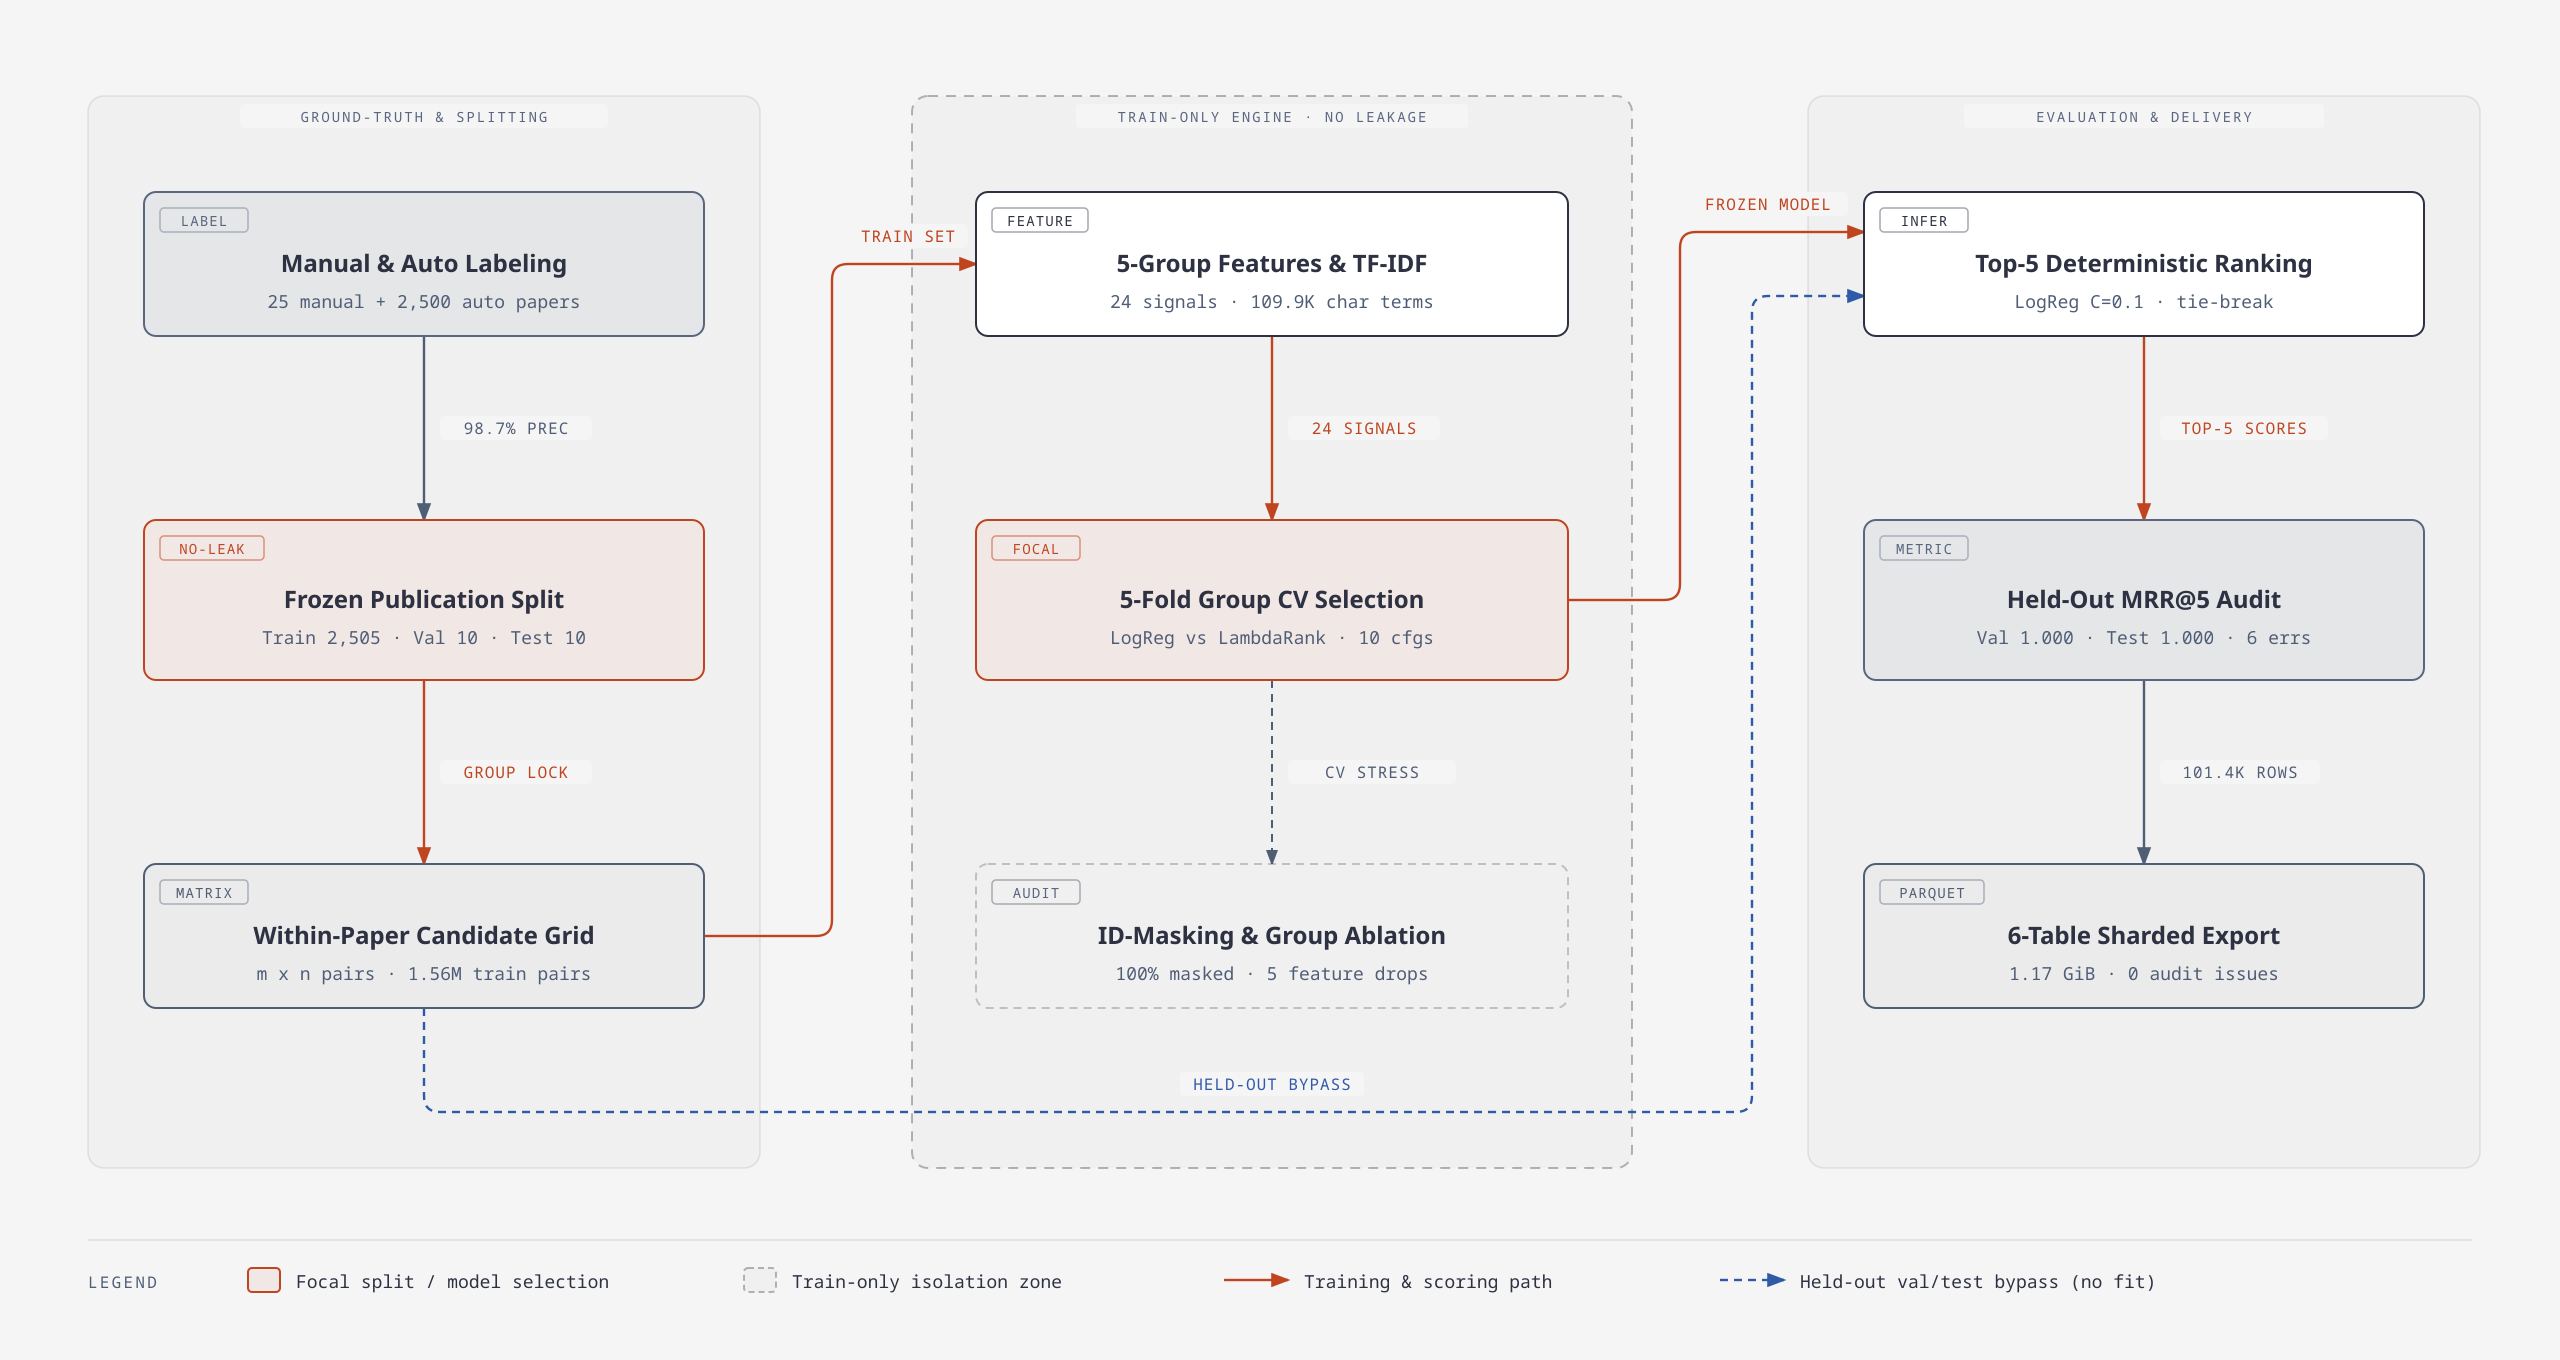
\includegraphics[width=\linewidth]{images/m3_matching_pipeline.png}
    \caption{Kiến trúc luồng xử lý Giai đoạn 3 từ dữ liệu đầu vào, tạo nhãn hai tầng, trích xuất 24 đặc trưng năm nhóm đến kiểm định chéo nhóm và xuất bản sáu bảng dữ liệu}
    \label{fig:m3_matching_pipeline}
\end{figure}

\subsection{Tiền xử lý văn bản và thiết kế hệ thống 24 đặc trưng}

Một quyết định thiết kế quan trọng của giai đoạn học máy là xây dựng dây chuyền chuẩn hóa văn bản độc lập hoàn toàn với bộ quy tắc gán nhãn tự động nhằm giảm thiểu rủi ro rò rỉ định kiến quy tắc vào biểu diễn đầu vào của mô hình. Trước khi tính toán bất kỳ độ đo tương đồng nào, tiêu đề của cả mục BibTeX lẫn tài liệu tham khảo arXiv đều đi qua chuỗi làm sạch gồm loại bỏ dấu phụ và lệnh ký tự Hy Lạp LaTeX, phân rã chuẩn hóa Unicode NFKD, chuyển về chữ thường và lọc từ dừng tiếng Anh thông dụng. Khác với nhiều bộ tiền xử lý ngôn ngữ tự nhiên phổ thông vốn loại bỏ mọi từ quá ngắn, bộ tách từ ở đây giữ nguyên toàn bộ ký hiệu toán học đơn ký tự và chữ số nhằm bảo toàn thông tin định danh đặc thù trong tiêu đề khoa học như tên đồ thị, nhóm đối xứng hay mức năng lượng. Đối với siêu dữ liệu tác giả, bộ phân tích họ tách riêng phần họ chuẩn hóa đồng thời xử lý đúng các hậu tố học thuật và tên các tổ chức hợp tác lớn trong vật lý năng lượng cao hay thiên văn học. Song song đó, bộ trích xuất mã định danh chỉ nhận diện mã arXiv khi đi kèm tiền tố ngữ cảnh tường minh của arXiv để tránh nhầm lẫn với số trang hay định danh tạp chí, còn năm công bố được trích xuất thống nhất về dạng số nguyên bốn chữ số.

Trên nền văn bản đã chuẩn hóa, mỗi cặp ứng viên $(e_i, r_j)$ trong cùng bài báo $p$ được mã hóa thành một vector gồm $24$ đặc trưng phân bổ vào năm nhóm ngữ nghĩa có tính bổ trợ chặt chẽ. Nhóm thứ nhất gồm $3$ đặc trưng định danh phản ánh trực tiếp trạng thái khớp mã arXiv: chỉ báo trùng khớp tuyệt đối mã arXiv giữa mục BibTeX và ứng viên, chỉ báo mục BibTeX có chứa mã arXiv tường minh, và chỉ báo xung đột mã định danh khi mục trích dẫn mang một mã arXiv xác định nhưng khác với mã của ứng viên đang xét. Nhóm thứ hai gồm $9$ đặc trưng từ vựng và tiểu từ trên tiêu đề nhằm bắt giữ đồng thời độ tương đồng cấp từ, độ bao hàm bất đối xứng khi một bên bị cắt ngắn và độ bền vững trước sai khác chính tả hay dấu gạch nối. Gọi $W_e$ và $W_r$ lần lượt là tập từ chuẩn hóa của tiêu đề mục BibTeX và ứng viên arXiv, ba độ đo tập hợp nền tảng gồm chỉ số Jaccard $J(W_e, W_r) = |W_e \cap W_r| / |W_e \cup W_r|$, tỷ lệ bao hàm chiều mục trích dẫn trong ứng viên $|W_e \cap W_r| / |W_e|$ và chiều ngược lại $|W_e \cap W_r| / |W_r|$. Bên cạnh hai độ tương đồng mờ theo tập từ và chuỗi con cục bộ, nhóm này bổ sung độ tương đồng cosin trên không gian vector TF-IDF $n$-gram ký tự độ dài $3$ đến $5$ với từ điển $109{,}864$ mục chỉ được khớp duy nhất trên tiêu đề tập huấn luyện để triệt tiêu rò rỉ thống kê. Ba đặc trưng còn lại của nhóm Tiêu đề là tỷ số độ dài tập từ giữa hai tiêu đề, chỉ báo trùng khớp chính xác tiêu đề chuẩn hóa và chỉ báo thiếu trường tiêu đề.

Ba nhóm đặc trưng còn lại cung cấp thông tin phân biệt ở tầng siêu dữ liệu đồng xuất hiện và cấu trúc cạnh tranh nội bài báo, giữ vai trò quyết định khi tiêu đề bị cắt xén hoặc nhiều bài báo cùng chuỗi sở hữu tiêu đề gần như trùng khít. Nhóm thứ ba gồm $4$ đặc trưng tác giả đo lường chỉ báo trùng khớp họ tác giả đầu tiên, chỉ số Jaccard trên tập họ tác giả, số lượng họ tác giả giao nhau tuyệt đối và chỉ báo thiếu trường tác giả. Việc giữ song song số lượng tác giả trùng lặp tuyệt đối bên cạnh chỉ số Jaccard đặc biệt hữu ích đối với các công trình hợp tác đông tác giả, nơi tỷ lệ Jaccard bị pha loãng khi tệp BibTeX rút gọn danh sách tác giả. Nhóm thứ tư gồm $3$ đặc trưng thời gian biểu diễn độ trễ công bố có dấu $\Delta y = y_e - y_r$, chỉ báo nằm trong ngưỡng sai lệch một năm $|\Delta y| \le 1$ và chỉ báo thiếu năm công bố. Giữ lại dấu của $\Delta y$ thay vì chỉ lấy giá trị tuyệt đối phản ánh đúng cơ chế xuất bản học thuật khi bản thảo nộp lên arXiv ở năm $y_r$ thường được đăng chính thức trên tạp chí hoặc hội nghị ở cùng năm hoặc năm kế tiếp ($\Delta y \in \{0, 1\}$). Nhóm thứ năm gồm $5$ đặc trưng cạnh tranh nội mục và liên mục trong bài báo $p$: thứ hạng tương đồng tiêu đề của ứng viên $r_j$ trong mục $e_i$, khoảng cách điểm so với ứng viên đứng đầu $g_{ij} = \max_{k} s(e_i, r_k) - s(e_i, r_j)$, điểm chuẩn hóa nội nhóm $z_{ij} = (s(e_i, r_j) - \mu_i) / \sigma_i$, chỉ báo song ánh tốt nhất hai chiều (bằng $1$ khi $r_j$ là ứng viên tiêu đề cao nhất của $e_i$ đồng thời $e_i$ là mục phù hợp nhất của $r_j$) và kích thước tập ứng viên $n_p$.

\begin{table}[htbp]
    \centering
    \scriptsize
    \renewcommand{\arraystretch}{1.14}
    \begin{tabularx}{\textwidth}{l X r r r l}
        \toprule
        \textbf{Nhóm} & \textbf{Đặc trưng (24 đặc trưng thuộc 5 nhóm)} & \textbf{TB (+)} & \textbf{TB (--)} & \textbf{AUC} & \textbf{Trọng số LR / Gain LGB nổi bật} \\
        \midrule
        \multirow{3}{*}{Định danh (3)}
            & Trùng khớp trực tiếp mã định danh arXiv & $0.2168$ & $0.0000$ & $0.6084$ & LR: $+3.244$; LGB: $35{,}143$ \\
            & Mục BibTeX có mã định danh arXiv tường minh & $0.2168$ & $0.2075$ & -- & LR: $-0.890$ \\
            & Xung đột mã định danh với ứng viên & $0.0000$ & $0.2075$ & $0.3962$ & LR: $-1.453$; LGB: $2{,}866$ \\
        \midrule
        \multirow{9}{*}{Tiêu đề (9)}
            & Chỉ số Jaccard tập từ tiêu đề $J(W_e, W_r)$ & $0.9788$ & $0.0538$ & $\mathbf{0.9964}$ & LR: $+1.882$; LGB: $1{,}842$ \\
            & Độ bao hàm từ tiêu đề mục trong ứng viên & $0.9826$ & $0.0958$ & $0.9954$ & LR: $-1.512$ \\
            & Độ bao hàm từ tiêu đề ứng viên trong mục & $0.9895$ & $0.0963$ & $0.9962$ & LGB: $2{,}269$ \\
            & Tương đồng mờ theo tập từ tiêu đề & $0.9951$ & $0.4462$ & $0.9950$ & -- \\
            & Tương đồng mờ theo chuỗi con cục bộ & $0.9948$ & $0.4759$ & $0.9956$ & -- \\
            & Cosin TF-IDF $n$-gram ký tự ($3$--$5$) & $0.9871$ & $0.1102$ & $0.9957$ & LR: $+1.515$ \\
            & Tỷ số độ dài tập từ hai tiêu đề & $0.9864$ & $0.7094$ & $0.9207$ & LR: $+0.885$; LGB: $2{,}428$ \\
            & Trùng khớp chính xác tiêu đề chuẩn hóa & $0.9431$ & $0.0000$ & $0.9715$ & LR: $+1.010$ \\
            & Chỉ báo thiếu trường tiêu đề & $0.0000$ & $0.0000$ & -- & -- \\
        \midrule
        \multirow{4}{*}{Tác giả (4)}
            & Trùng khớp họ tác giả đầu tiên & $0.9650$ & $0.0144$ & $0.9753$ & LGB: $1{,}469$ \\
            & Chỉ số Jaccard tập họ tác giả & $0.9086$ & $0.0234$ & $\mathbf{0.9862}$ & LGB: $697$ \\
            & Số lượng họ tác giả trùng lặp & $5.419$ & $0.262$ & $0.9722$ & -- \\
            & Chỉ báo thiếu danh sách tác giả & $0.0020$ & $0.0024$ & -- & -- \\
        \midrule
        \multirow{3}{*}{Thời gian (3)}
            & Chênh lệch năm công bố có dấu $\Delta y$ & $0.411$ & $0.447$ & -- & LGB: $1{,}759$ \\
            & Chỉ báo sai lệch trong vòng một năm $|\Delta y| \le 1$ & $0.9193$ & $0.3293$ & $0.7950$ & LR: $+0.841$ \\
            & Chỉ báo thiếu trường năm công bố & $0.0097$ & $0.0061$ & -- & -- \\
        \midrule
        \multirow{5}{*}{Cạnh tranh (5)}
            & Thứ hạng tiêu đề trong nội bộ mục truy vấn & $1.096$ & $35.146$ & $0.9978^*$ & LGB: $\mathbf{3{,}309{,}532}$ \\
            & Khoảng cách điểm so với ứng viên đứng đầu $g_{ij}$ & $0.0007$ & $0.5502$ & $\mathbf{0.9989^*}$ & LR: $\mathbf{-3.317}$; LGB: $160{,}866$ \\
            & Điểm chuẩn hóa nội mục $z_{ij}$ & $+4.339$ & $-0.098$ & $0.9956$ & LR: $+1.167$; LGB: $1{,}085$ \\
            & Tín hiệu song ánh tốt nhất hai chiều & $0.9907$ & $0.0012$ & $0.9947$ & -- \\
            & Kích thước tập ứng viên của bài báo $n_p$ & $45.49$ & $68.60$ & -- & LR: $-1.957$ \\
        \bottomrule
    \end{tabularx}
    \caption[Thống kê phân tách 24 đặc trưng trên 1{,}561{,}952 cặp ứng viên huấn luyện]{Thống kê phân tách 24 đặc trưng trên $1{,}561{,}952$ cặp ứng viên huấn luyện (TB (+)/(--): trung bình lớp dương/âm; dấu $^*$ biểu thị ROC-AUC đảo chiều $1 - \text{AUC}$ cho các đặc trưng có tương quan nghịch với xác suất khớp; ký hiệu ``--'' ứng với các hệ số phụ hoặc đa cộng tuyến không thuộc nhóm dẫn đầu).}
    \label{tab:m3_features}
\end{table}

Thống kê thực nghiệm trên toàn bộ $1{,}561{,}952$ cặp ứng viên huấn luyện tại Bảng~\ref{tab:m3_features} minh họa mức độ phân tách rõ rệt của hệ thống đặc trưng thiết kế, đồng thời làm nổi bật sự khác biệt trong cách khai thác tín hiệu giữa mô hình tuyến tính và mô hình cây quyết định. Xét đơn biến theo chỉ số ROC-AUC, hai đặc trưng cạnh tranh nội nhóm dẫn đầu tuyệt đối với khoảng cách so với ứng viên đứng đầu đạt $0.9989$ (đảo chiều từ $0.0011$, trung bình $0.0007$ ở lớp dương so với $0.5502$ ở lớp âm) và thứ hạng tiêu đề nội mục đạt $0.9978$ (đảo chiều từ $0.0022$, trung bình $1.096$ so với $35.146$). Theo sát ngay sau là nhóm đặc trưng tiêu đề và tác giả, nổi bật là chỉ số Jaccard tập từ ($0.9964$), độ bao hàm ứng viên trong mục ($0.9962$), cosin TF-IDF ký tự ($0.9957$) và Jaccard họ tác giả ($0.9862$). Ở Hồi quy Logistic chuẩn hóa, khoảng cách so với ứng viên đứng đầu nhận trọng số âm mạnh nhất ($-3.317$) và trùng khớp mã định danh nhận trọng số dương lớn nhất ($+3.244$), trong khi xung đột mã định danh mang trọng số phạt $-1.453$ và kích thước tập ứng viên mang trọng số hiệu chỉnh nền $-1.957$. Đáng chú ý, độ bao hàm chiều mục trong ứng viên nhận dấu âm ($-1.512$) bên cạnh Jaccard ($+1.882$) và TF-IDF ký tự ($+1.515$) như một thành phần cân bằng đa cộng tuyến nhằm phạt các tiêu đề quá ngắn vô tình lọt trọn vào một tiêu đề dài hơn. Ngược lại, ở mô hình LightGBM LambdaRank, thứ hạng tiêu đề nội mục chiếm ưu thế áp đảo về độ lợi chia nhánh ($3{,}309{,}532$), theo sau là khoảng cách so với ứng viên đứng đầu ($160{,}866$) và trùng khớp mã định danh ($35{,}143$), cho thấy cấu trúc cây phân tầng đặt thứ hạng nội nhóm làm trục phân tách gốc rồi tinh chỉnh các ca tranh chấp bằng mã định danh, tỷ số độ dài tiêu đề, chênh lệch năm có dấu và họ tác giả đầu tiên.

\subsection{Quy trình huấn luyện, kiểm định chéo, kịch bản che mã định danh và kết quả MRR@5}

Hiệu năng xếp hạng của toàn bộ mô hình được đo lường bằng chỉ số Thứ hạng nghịch đảo trung bình trong tốp năm ứng viên đầu tiên ($\text{MRR@5}$)~\cite{craswell2009}, định nghĩa trên tập truy vấn có nhãn đúng $Q$ theo Công thức~\eqref{eq:mrr5}:
\begin{equation}
    \text{MRR@5} = \frac{1}{|Q|} \sum_{i=1}^{|Q|} \mathbb{I}(\text{rank}_i \le 5)\,\frac{1}{\text{rank}_i},
    \label{eq:mrr5}
\end{equation}
trong đó $\text{rank}_i \in \{1, \dots, n_p\}$ là vị trí của tài liệu tham khảo đích $r^*_i$ sau khi sắp xếp toàn bộ ứng viên của bài báo $p$ theo điểm dự đoán giảm dần, còn hàm chỉ thị $\mathbb{I}(\text{rank}_i \le 5)$ gán giá trị $0$ cho mọi truy vấn có đích đúng rơi ra ngoài năm hạng đầu. Tuân thủ quy ước đánh giá thống nhất của học phần~\cite{hcmus_intro_ds}, mẫu số $|Q|$ bao gồm tất cả các mục BibTeX đã xác minh có tài liệu tham khảo đích tồn tại trong kho arXiv của bài báo ($35{,}373$ truy vấn toàn cục). Trong khi đó, bảng kết quả dự đoán phát hành vẫn cung cấp đầy đủ năm ứng viên xếp hạng cao nhất cho toàn bộ $101{,}441$ mục thuộc tập đối sánh và để trống trường mã đích chuẩn đối với các mục không có đích khớp hoặc chưa rà soát. Xuyên suốt quy trình huấn luyện, nguyên tắc chống rò rỉ dữ liệu được áp dụng tuyệt đối ở mọi tầng xử lý. Bộ biến đổi TF-IDF $n$-gram ký tự, bộ chuẩn hóa tỷ lệ đặc trưng và các tham số mô hình đều chỉ được khớp trên tập huấn luyện (hoặc từng nếp huấn luyện trong kiểm định chéo), còn tập kiểm tra $10$ bài báo ($528$ truy vấn) bị niêm phong hoàn toàn cho đến sau khi chốt mô hình duy nhất.

Quá trình lựa chọn mô hình triển khai kiểm định chéo năm nếp phân nhóm theo bài báo (5-fold Group K-Fold) trên $2{,}505$ bài báo huấn luyện ($34{,}334$ truy vấn), khảo sát lưới $10$ cấu hình gồm $3$ mức điều chuẩn của Hồi quy Logistic ($C \in \{0.1, 1.0, 10.0\}$) và $2$ mức dung lượng của LightGBM LambdaRank ($15$ và $31$ lá). Mỗi mô hình được thử nghiệm song song ở hai chế độ không tăng cường và có tăng cường dữ liệu che mã định danh tất định với xác suất $50\%$, tức cố ý ẩn nhóm đặc trưng mã arXiv trên một nửa truy vấn huấn luyện để buộc mô hình học sâu hơn từ tiêu đề, tác giả và năm công bố. Ngoài kịch bản đánh giá bình thường, mọi cấu hình đều phải trải qua bài kiểm tra áp lực che $100\%$ mã định danh nhằm đo khả năng tổng quát hóa khi gặp các mục BibTeX hoàn toàn thiếu mã arXiv. Trên tập con $1{,}014$ truy vấn thủ công nằm trong phần huấn luyện, cả $10$ cấu hình đều đạt điểm tuyệt đối $1.0000$ ở cả hai kịch bản, qua đó kích hoạt quy tắc phân giải hòa theo độ phức tạp ưu tiên mô hình tuyến tính gọn nhẹ và điều chuẩn mạnh nhất là Hồi quy Logistic ($C = 0.1$, không tăng cường). Khi mở rộng đánh giá sang toàn bộ $34{,}334$ truy vấn kiểm định chéo như tổng hợp tại Bảng~\ref{tab:m3_results}, Hồi quy Logistic ($C = 0.1$) dẫn đầu điểm kiểm định chéo bình thường ở mức $0.999898$. Đáng chú ý, việc bật tăng cường che $50\%$ mã định danh giúp Hồi quy Logistic ($C = 10.0$) nâng điểm kiểm định chéo che mã từ $0.997018$ lên $0.998662$, và đặc biệt đẩy LightGBM LambdaRank ($31$ lá) đạt $0.999100$---cắt giảm xấp xỉ $70\%$ tỷ lệ sai số xếp hạng trong điều kiện vắng mã định danh mà vẫn duy trì điểm bình thường ở mức $0.999869$.

\begin{table}[htbp]
    \centering
    \scriptsize
    \renewcommand{\arraystretch}{1.18}
    \begin{tabularx}{\textwidth}{X c c c c c}
        \toprule
        \textbf{Mô hình / Cấu hình đánh giá} & \textbf{CV Thường} & \textbf{CV Che ID} & \textbf{Valid ($n=511$)} & \textbf{Test ($n=528$)} & \textbf{Toàn cục ($35{,}373$)} \\
        \midrule
        Đường cơ sở (tương đồng tập từ tiêu đề) & -- & -- & $0.9780$ ($0.9741^\dagger$) & $0.9981$ ($0.9977^\dagger$) & $0.9848$ ($905$ lỗi) \\
        \midrule
        \textbf{LR ($C=0.1$, không tăng cường) [Đã chọn]} & $\mathbf{0.999898}$ & $0.997018$ & $\mathbf{1.0000}$ & $\mathbf{1.0000}$ & $\mathbf{0.999901}$ ($6$ lỗi) \\
        LR ($C=10.0$, tăng cường che $50\%$ ID) & $0.999840$ & $0.998662$ & -- & -- & -- \\
        LightGBM LambdaRank ($15$ lá, không tăng cường) & $0.999869$ & $0.997054$ & -- & -- & -- \\
        LightGBM LambdaRank ($31$ lá, tăng cường che $50\%$ ID) & $0.999869$ & $\mathbf{0.999100}$ & $\mathbf{1.0000}$ & $\mathbf{1.0000}$ & -- \\
        \bottomrule
    \end{tabularx}
    \caption[So sánh chỉ số MRR@5 giữa đường cơ sở và các cấu hình học máy]{So sánh chỉ số MRR@5 giữa đường cơ sở và các cấu hình học máy trên kiểm định chéo $5$ nếp ($n=34{,}334$), tập kiểm định, tập kiểm tra và toàn bộ kho nhãn (giá trị mang dấu $^\dagger$ biểu thị điểm riêng trên phân tập nhãn thủ công của đường cơ sở; trên Valid và Test, mô hình được chọn đạt $1.0000$ ở cả chế độ thường lẫn che $100\%$ mã định danh).}
    \label{tab:m3_results}
\end{table}

Trên hai tập đánh giá độc lập, mô hình Hồi quy Logistic được chọn mang lại mức cải thiện rõ rệt so với đường cơ sở chỉ dựa trên tương đồng tập từ tiêu đề. Đường cơ sở đạt MRR@5 bằng $0.9780$ trên tập kiểm định ($0.9741$ trên phần thủ công và $1.0000$ trên phần tự động; tỷ lệ khớp đúng hạng nhất $95.69\%$, tốp ba $99.80\%$ và tốp năm $100.0\%$) và đạt $0.9981$ trên tập kiểm tra ($0.9977$ trên phần thủ công và $1.0000$ trên phần tự động; hạng nhất $99.62\%$, tốp ba và tốp năm $100.0\%$). Khi mở rộng ra toàn bộ $35{,}373$ truy vấn, hạn chế của tiêu chí chỉ xét tiêu đề bộc lộ rõ với điểm MRR@5 dừng ở $0.9848$ kèm $905$ trường hợp trượt khỏi hạng nhất, bao gồm $669$ trường hợp ở hạng $2$, $73$ ở hạng $3$, $16$ ở hạng $4$, $19$ ở hạng $5$ và $128$ trường hợp rơi hoàn toàn khỏi tốp năm. Ngược lại, mô hình Hồi quy Logistic ($C=0.1$) đạt MRR@5 tuyệt đối $1.0000$ trên cả $511$ truy vấn kiểm định lẫn $528$ truy vấn kiểm tra với $0$ sai số, đồng thời bảo toàn trọn vẹn mức $1.0000$ ngay cả khi che $100\%$ mã arXiv. Cấu hình LightGBM LambdaRank ($31$ lá, có tăng cường che mã) cũng tái lập mức $1.0000$ tương đương trên cả hai phân vùng độc lập này. Tính trên toàn bộ $35{,}373$ truy vấn, mô hình được chọn đạt MRR@5 bằng $0.999901$ với tỷ lệ khớp đúng hạng nhất lên đến $99.983\%$ và tỷ lệ trong tốp ba cũng như tốp năm đạt $99.997\%$, chỉ ghi nhận đúng $6$ bất đồng trên toàn bộ kho dữ liệu (gồm $5$ trường hợp ở hạng $2$ và $1$ trường hợp ngoài tốp năm, toàn bộ đều nằm trong phần tự động của tập huấn luyện).

\begin{figure}[htbp]
    \centering
    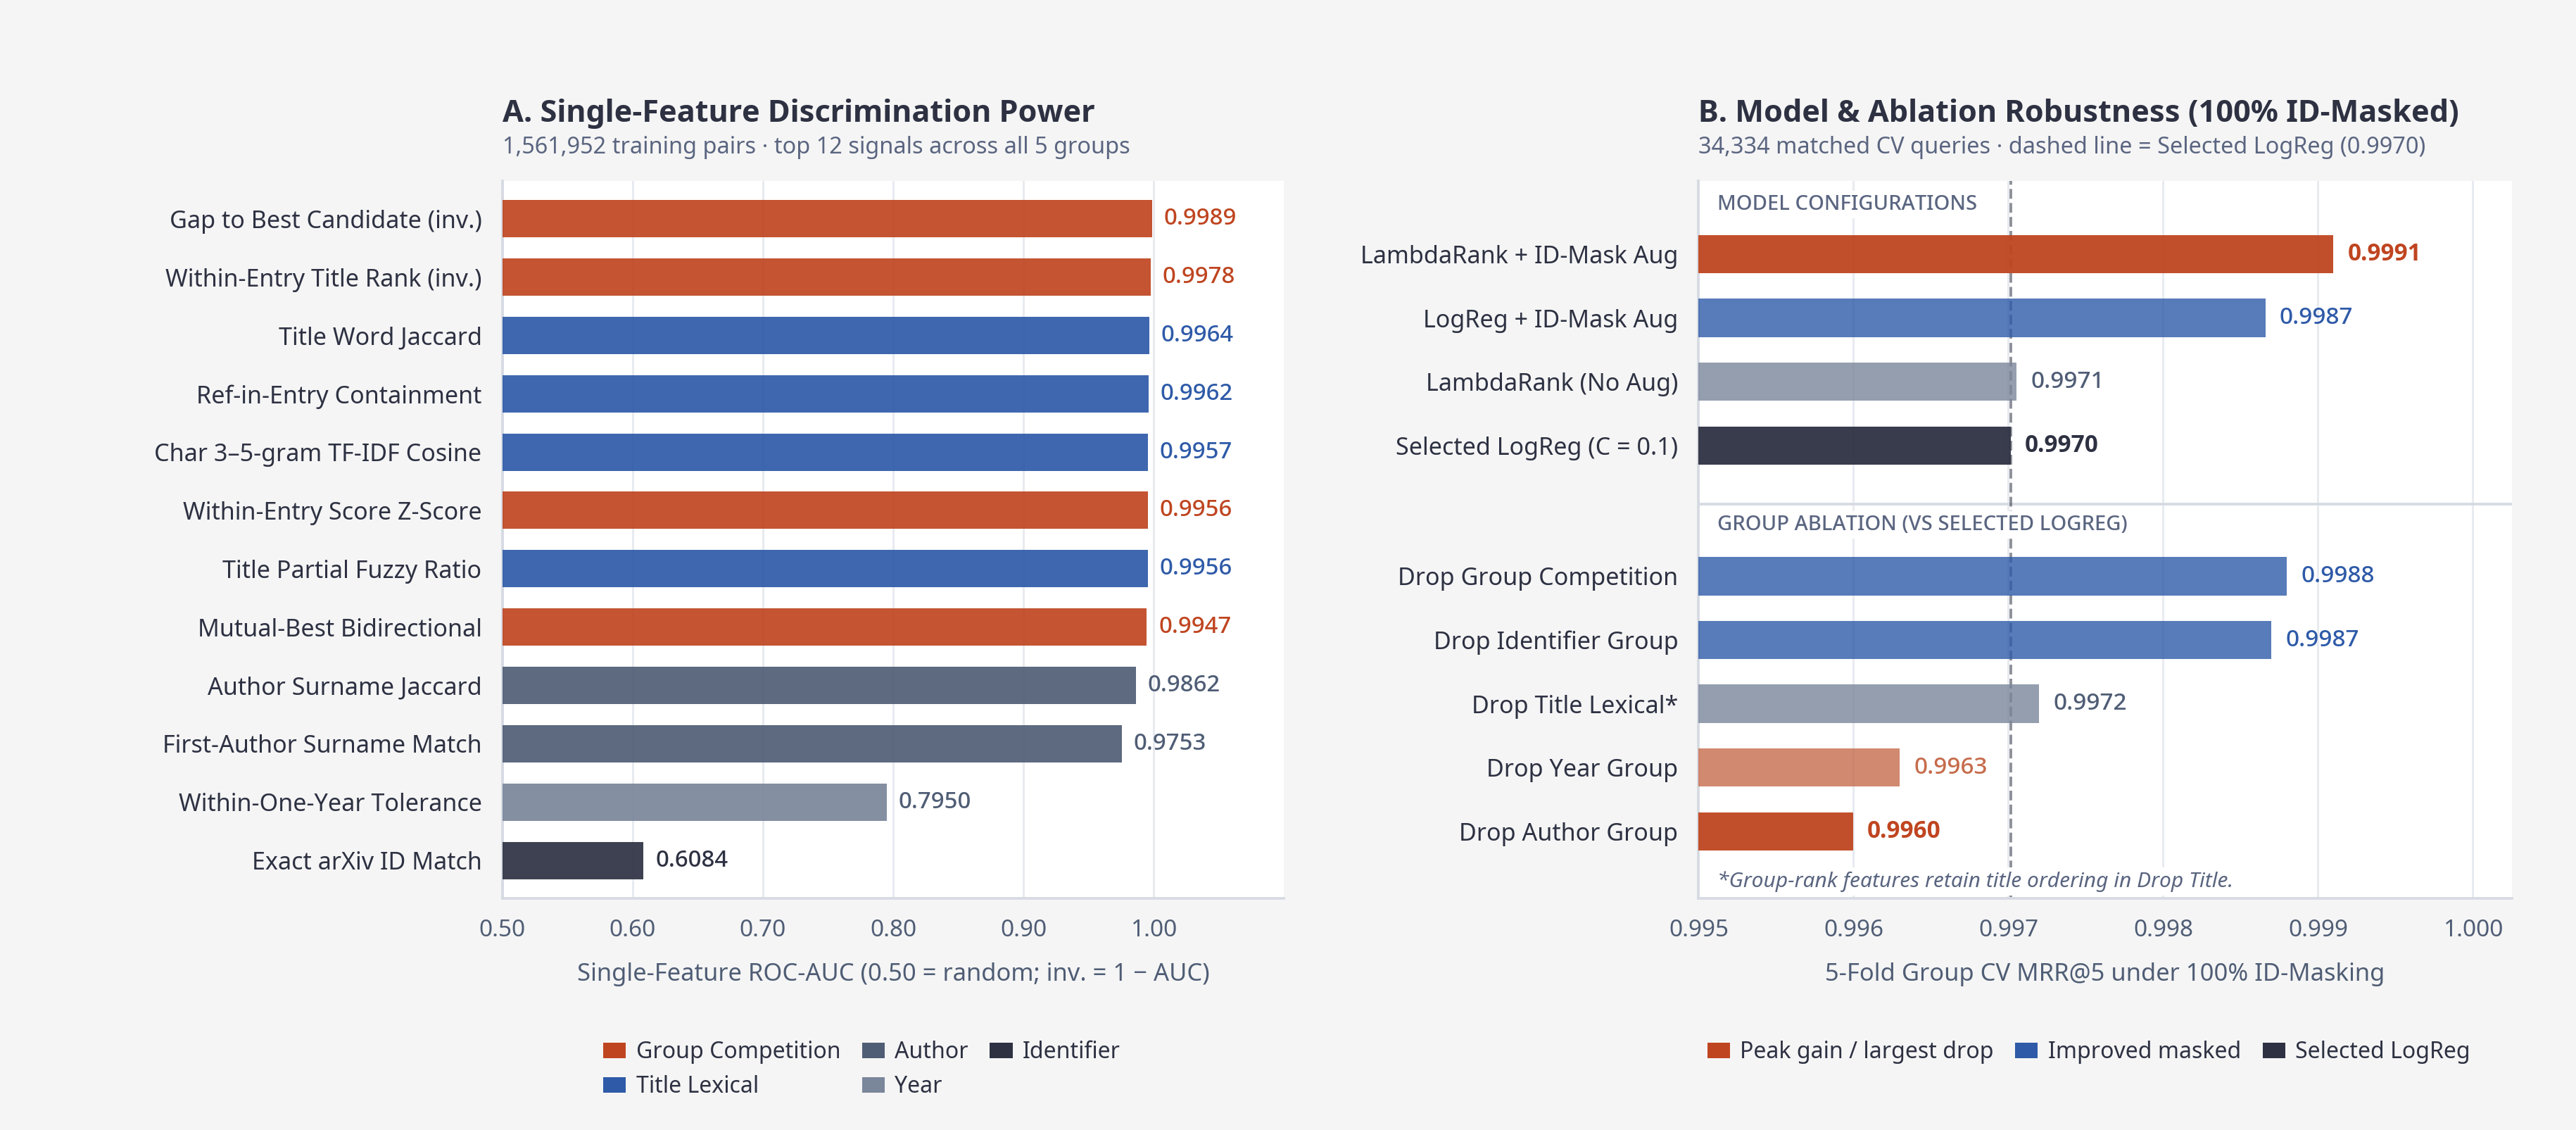
\includegraphics[width=\linewidth]{images/m3_feature_ablation.png}
    \caption[Năng lực phân tách đặc trưng và thí nghiệm loại trừ nhóm đặc trưng]{Đánh giá năng lực phân tách của các nhóm đặc trưng và kết quả thí nghiệm loại trừ từng nhóm đặc trưng trên kiểm định chéo $5$ nếp ($34{,}334$ truy vấn) dưới hai kịch bản bình thường và che $100\%$ mã định danh.}
    \label{fig:m3_feature_ablation}
\end{figure}

Để kiểm chứng đóng góp biên thực sự của từng nhóm tín hiệu, nhóm tiến hành nghiên cứu loại trừ lần lượt từng nhóm đặc trưng trên toàn bộ $34{,}334$ truy vấn kiểm định chéo như minh họa tại Hình~\ref{fig:m3_feature_ablation}. So với cấu hình đầy đủ đạt $0.9999$ ở chế độ bình thường và $0.9970$ ở chế độ che mã định danh, việc loại bỏ nhóm Tác giả gây sụt giảm mạnh nhất dưới kịch bản che mã xuống còn $0.9960$, theo sát ngay sau là việc loại bỏ nhóm Thời gian làm giảm điểm che mã xuống $0.9963$. Kết quả thực nghiệm này chứng minh siêu dữ liệu tác giả và độ trễ năm công bố đóng vai trò phân giải chủ lực khi các mục trích dẫn thiếu mã arXiv. Hai phát hiện nghịch trực giác nhưng nhất quán về mặt cơ chế cũng xuất hiện rõ ràng trong bảng loại trừ: khi loại bỏ nhóm Định danh ngay từ lúc huấn luyện, điểm bình thường giảm nhẹ về $0.9987$ nhưng điểm che mã lại tăng từ $0.9970$ lên $0.9987$ vì mô hình buộc phải phân bổ trọng số đồng đều cho văn bản và siêu dữ liệu thay vì ỷ lại vào mã arXiv. Tương tự, việc loại bỏ nhóm Cạnh tranh giúp điểm che mã tăng lên $0.9988$ do hạn chế hiện tượng quá phụ thuộc vào thứ hạng tiêu đề thô trong các tình huống tiêu đề bị cắt ngắn. Cần ghi nhận một điểm tinh tế về phương pháp luận ở nhánh loại trừ nhóm Tiêu đề ($0.9992$ bình thường, phân tập thủ công giảm về $0.9992$, và $0.9972$ che mã): do các đặc trưng thứ hạng, khoảng cách tốt nhất và điểm chuẩn hóa trong nhóm Cạnh tranh vẫn được tính từ điểm tương đồng tiêu đề gốc, thông tin thứ tự tiêu đề vẫn gián tiếp lưu lại trong biểu diễn sau khi rút nhóm Tiêu đề.

Về chi phí tính toán và kiểm chứng xuất bản, toàn bộ dây chuyền Giai đoạn 3 cho cả năm thành viên hoàn tất trọn vẹn trên $2$ luồng CPU trong tổng thời gian $772.85\text{ s}$ ($12.88\text{ phút}$) với mức tiêu thụ bộ nhớ đỉnh $2{,}393.5\text{ MB}$. Trong tổng thời lượng này, công đoạn huấn luyện và chọn mô hình tiêu tốn $476.26\text{ s}$, phân bổ chủ yếu vào kiểm định chéo $10$ cấu hình trên $5$ nếp ($407.85\text{ s}$) và trích xuất đặc trưng tập huấn luyện ($30.25\text{ s}$), còn bước khớp lại mô hình Hồi quy Logistic cuối cùng chỉ mất đúng $1.81\text{ s}$. Kết quả đầu ra của cả năm thành viên được đóng gói theo định dạng cột Apache Parquet phân mảnh~\cite{apache_parquet} thành sáu bảng chuẩn có tổng dung lượng $1{,}199.45\text{ MiB}$ ($1.171\text{ GiB}$). Cụ thể, kho dữ liệu bao gồm bảng siêu dữ liệu bài báo ($25{,}000$ dòng, $3.73\text{ MiB}$), bảng tài liệu tham khảo ($466{,}763$ dòng, $75.01\text{ MiB}$), bảng phần tử nội dung ($11{,}098{,}189$ dòng, $902.35\text{ MiB}$), bảng quan hệ phân cấp ($16{,}185{,}255$ dòng, $88.50\text{ MiB}$), bảng mục lục BibTeX ($975{,}674$ dòng, $126.41\text{ MiB}$) và bảng kết quả dự đoán đối sánh ($101{,}441$ dòng, $3.44\text{ MiB}$). Toàn bộ bộ dữ liệu phát hành của cả năm thành viên đều vượt qua quy trình kiểm định tự động độc lập về lược đồ cột, tính duy nhất khóa chính, toàn vẹn khóa ngoại liên bảng và quy tắc thứ hạng tốp năm với $0$ lỗi được phát hiện.

\subsection{Phân tích lỗi chuyên sâu trên toàn bộ 35{,}373 truy vấn}

Vì mô hình Hồi quy Logistic được chọn đạt $0$ sai số trên cả hai tập kiểm định độc lập và chỉ tạo ra đúng $6$ bất đồng trên toàn bộ $35{,}373$ truy vấn có nhãn, nhóm có điều kiện thực hiện kiểm định thủ công toàn diện từng trường hợp mà không cần lấy mẫu xấp xỉ. Quy trình rà soát đối chiếu trực tiếp nội dung mục BibTeX gốc, toàn bộ tập ứng viên arXiv của bài báo trích dẫn và bản gốc công trình khoa học tương ứng để xác định nguyên nhân gốc. Kết quả phân loại tổng hợp tại Bảng~\ref{tab:m3_error_forensics} cho thấy toàn bộ $6$ trường hợp bất đồng đều nằm trong phân vùng tự động của tập huấn luyện, trong đó có tới $4$ trường hợp bắt nguồn từ nhiễu nhãn của bộ quy tắc tự động và $1$ trường hợp xuất phát từ lỗi phân tích cú pháp mục tham khảo ngược dòng từ Giai đoạn 2. Chỉ có duy nhất $1$ trong $6$ bất đồng thực sự là sai sót xếp hạng của mô hình học máy, và ngay trong trường hợp đó tài liệu đích vẫn được xếp sát nút ở hạng $2$. Phân rã này chứng tỏ mô hình tuyến tính điều chuẩn mạnh đã không học vẹt các sai sót hệ thống của nhãn giám sát yếu, mà trái lại đã khái quát hóa chính xác hơn chính bộ quy tắc tạo nhãn huấn luyện của nó.

\begin{table}[htbp]
    \centering
    \scriptsize
    \renewcommand{\arraystretch}{1.18}
    \begin{tabularx}{\textwidth}{c p{0.23\textwidth} c X}
        \toprule
        \textbf{TT} & \textbf{Phân loại nguyên nhân gốc} & \textbf{Hạng nhãn} & \textbf{Bản chất kỹ thuật và ứng xử của mô hình học máy} \\
        \midrule
        1 & Nhiễu nhãn tự động (mô hình sửa đúng) & Hạng $2$ & Bài báo về số bão hòa đồ thị $C_6$ ($2021$): quy tắc loại bỏ từ $2$ ký tự làm ghép nhầm vào bài báo $W_4$ ($2025$); mô hình khôi phục đúng bài $C_6$ nhờ trùng cả bốn tác giả. \\
        2 & Nhiễu nhãn tự động (mô hình sửa đúng) & Hạng $2$ & Bài báo ATLAS $7\text{ TeV}$ ($2014$): quy tắc ghép nhầm sang bài ATLAS $8\text{ TeV}$ ($2016$); mô hình chọn đúng bài $2014$ nhờ khớp tác giả đầu và năm công bố dù tiêu đề bị cắt ngắn. \\
        3 & Nhiễu nhãn tự động (mô hình sửa đúng) & Hạng $2$ & Bài báo hố đen siêu đối xứng của Gutowski và Reall ($2004$): quy tắc ghép nhầm sang bài năm $2006$ của nhóm Kunduri--Lucietti--Reall qua một đồng tác giả; mô hình chọn đúng bài $2004$. \\
        4 & Mục không có đích khớp bị gán nhãn sai & Ngoài tốp $5$ & Bài báo mã lượng tử MDS ($2014$) thực tế không nằm trong tập tham khảo arXiv đã thu hoạch; quy tắc gán nhầm vào bài năm $2014$ khác có chung họ tác giả Zhu, còn mô hình bác bỏ ứng viên sai này. \\
        5 & Lỗi phân tích mục tham khảo Giai đoạn 2 & Hạng $2$ & Mục tham khảo dùng ký hiệu gạch ngang lặp tác giả kèm DOI tạp chí thiên văn nhúng mã $2311.03286$ không có tiền tố arXiv tường minh; quy tắc bắt được dãy số trong khi bộ trích xuất học máy bỏ qua và gặp tiêu đề lỗi. \\
        6 & Lỗi xếp hạng thực sự của mô hình & Hạng $2$ & Bài báo năng lượng tối Barrow ($2021$) viết từ ghép liền (``nonflat'') đối đầu bản có gạch nối (``non-flat'') và bài tiền nhiệm ngắn hơn năm $2020$ đạt bao hàm chuỗi con toàn phần; đích đúng vẫn đứng hạng $2$. \\
        \bottomrule
    \end{tabularx}
    \caption{Phân tích nguyên nhân gốc của toàn bộ $6$ trường hợp bất đồng trên tổng số $35{,}373$ truy vấn}
    \label{tab:m3_error_forensics}
\end{table}

Bốn trường hợp đầu tiên minh họa rõ lợi ích của việc kết hợp đa tín hiệu tác giả, thời gian và bảo toàn ký hiệu ngắn thay vì dựa vào ngưỡng quy tắc cứng. Ở trường hợp thứ nhất về bài báo số bão hòa của đồ thị $C_6$ năm $2021$, bộ quy tắc tự động loại bỏ các từ ngắn hai ký tự khiến cả $C_6$ lẫn $W_4$ biến mất khỏi tiêu đề, dẫn tới ghép nhầm vào một công trình năm $2025$ nghiên cứu đồ thị $W_4$. Trái lại, mô hình học máy giữ nguyên ký hiệu ngắn và khai thác sự trùng khớp trọn vẹn của cả bốn tác giả để xếp đúng bài báo năm $2021$ lên hạng nhất. Ở trường hợp thứ hai liên quan đến đo đạc tiết diện toàn phần của thực nghiệm ATLAS tại năng lượng $7\text{ TeV}$ năm $2014$, tiêu đề lưu trên Semantic Scholar bị cắt ngắn làm tầng mờ của bộ quy tắc nghiêng về bài báo ATLAS $8\text{ TeV}$ năm $2016$, trong khi mô hình học máy dựa vào sự trùng khớp chặt giữa tác giả đầu tiên và năm công bố $2014$ để khôi phục chính xác tài liệu đích. Tương tự, ở trường hợp thứ ba về công trình hố đen siêu đối xứng trong không gian năm chiều của Gutowski và Reall năm $2004$, bộ quy tắc tự động bị đánh lừa bởi một đồng tác giả chung và ghép sang bài báo năm $2006$ của Kunduri, Lucietti và Reall, còn mô hình học máy đưa đúng bài báo gốc năm $2004$ lên vị trí dẫn đầu. Ở trường hợp thứ tư---cũng là trường hợp duy nhất nhãn tự động rơi ra ngoài tốp năm---công trình năm $2014$ về mã lượng tử MDS vốn vắng mặt hoàn toàn trong tập tham khảo arXiv của bài báo trích dẫn nhưng bị bộ quy tắc tự động gán nhầm vào một bài báo mã học khác cùng năm có chung họ tác giả Zhu, cho thấy mô hình đã loại trừ đúng ứng viên nhiễu.

Hai trường hợp cuối cùng chỉ ra trực tiếp các giới hạn kỹ thuật cụ thể ở tầng phân tích cú pháp ngược dòng và tiền xử lý từ ghép. Ở trường hợp thứ năm, nguyên nhân nằm hoàn toàn ở đầu vào của Giai đoạn 2: một mục tham khảo nội tuyến trong vật lý thiên văn dùng quy ước gạch ngang thay thế tên tác giả lặp lại đồng thời nhúng mã $2311.03286$ vào trong mã DOI của tạp chí mà không viết từ khóa arXiv tường minh. Vì vậy, bộ quy tắc tự động vẫn bắt được dãy mã số trong khi bộ phân tích học máy nghiêm ngặt bỏ qua chuỗi số thiếu ngữ cảnh và buộc phải xếp hạng dựa trên chuỗi tiêu đề bị hỏng cấu trúc. Chỉ duy nhất trường hợp thứ sáu là sai lầm xếp hạng thực chất của mô hình tuyến tính khi xử lý biến thể chính tả từ ghép. Cụ thể, mục BibTeX trích dẫn công trình năm $2021$ về năng lượng tối toàn ảnh Barrow trong vũ trụ không phẳng bằng cách viết liền không gạch nối (``nonflat''), trong khi siêu dữ liệu Semantic Scholar ghi dạng có gạch nối (``non-flat''), khiến điểm trùng khớp từ vựng bị giảm tương đối so với bài báo tiền nhiệm năm $2020$ có tiêu đề ngắn hơn đạt bao hàm chuỗi con trọn vẹn. Dù chịu bất lợi chính tả này, mô hình vẫn giữ tài liệu đúng năm $2021$ ở vị trí thứ hai sát nút, đưa tỷ lệ sai sót xếp hạng thực chất trên toàn bộ $35{,}373$ truy vấn về đúng $1/35{,}373$.
